%% This is an example first chapter.  You should put chapter/appendix that you
%% write into a separate file, and add a line \include{yourfilename} to
%% main.tex, where `yourfilename.tex' is the name of the chapter/appendix file.
%% You can process specific files by typing their names in at the 
%% \files=
%% prompt when you run the file main.tex through LaTeX.

\singlespacing{

\chapter{Future Work}\label{chap:futureWork}

\section{Hierarchical Simulation}

\section{"Fab the Game"}

\begin{figure}
  \includegraphics[width=\textwidth]{elibendy.png}
  \caption{\textit{Image Credit: Eli Gershenfeld 2016}}
  \label{fig:elibendy}
\end{figure}

\begin{figure}
  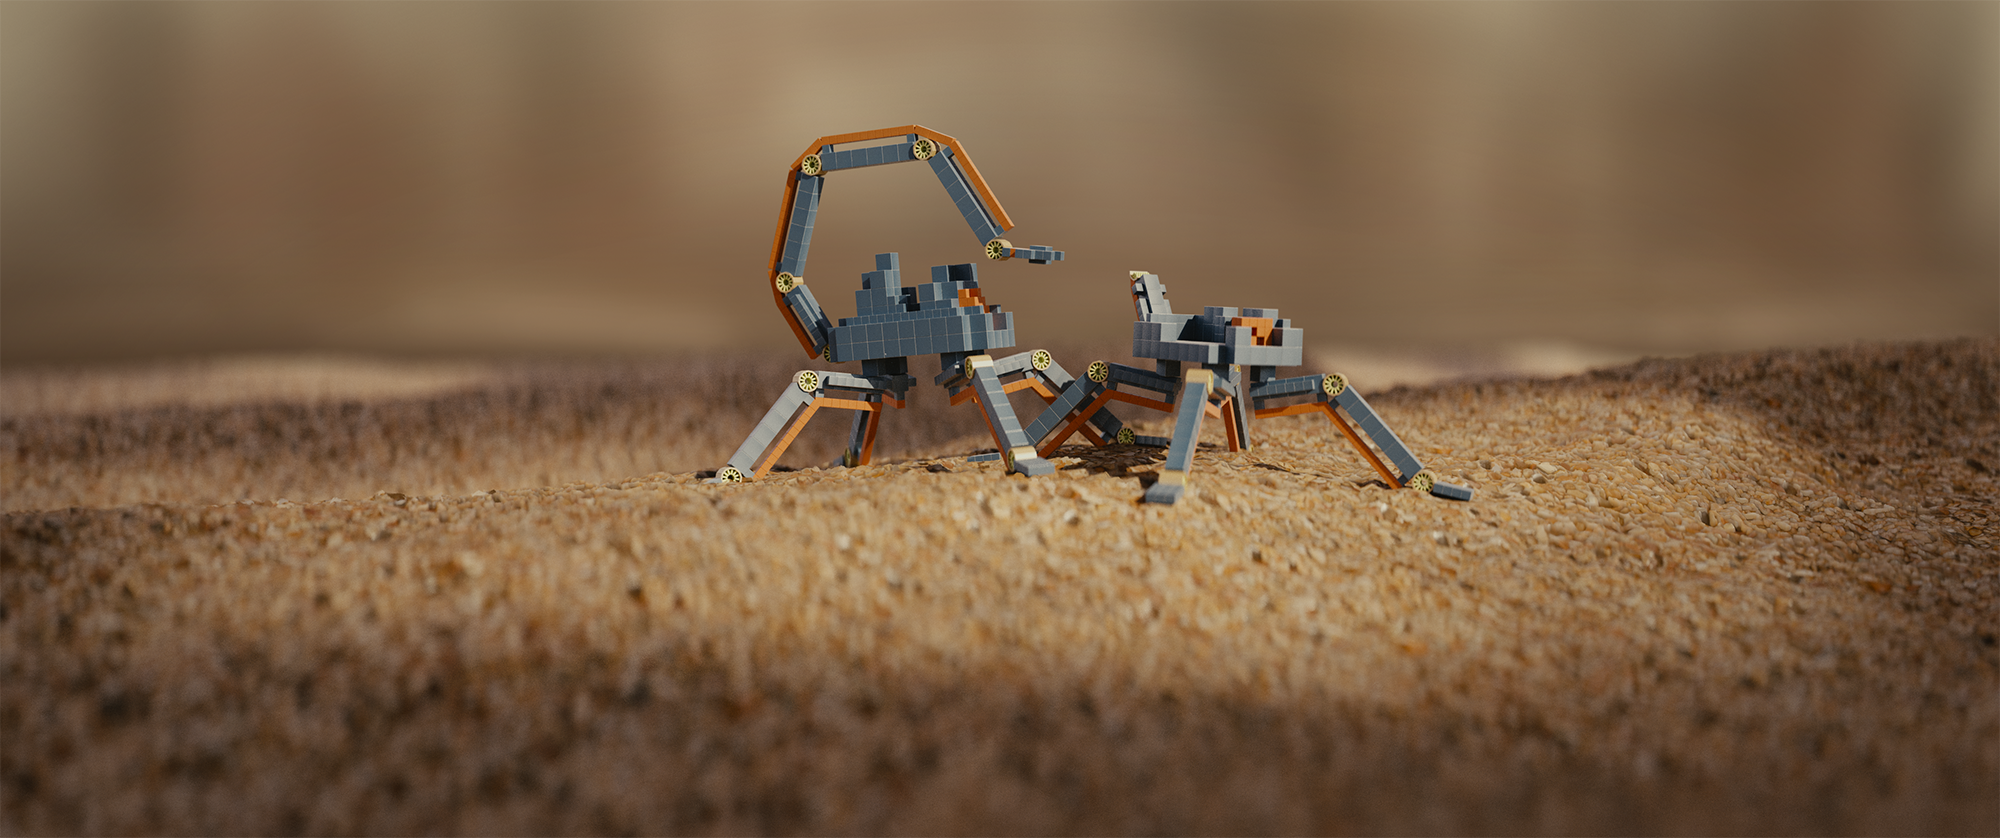
\includegraphics[width=\textwidth]{eliassemblers.png}
  \caption{\textit{Image Credit: Eli Gershenfeld 2016}}
  \label{fig:eliassemblers}
\end{figure}

\begin{figure}
  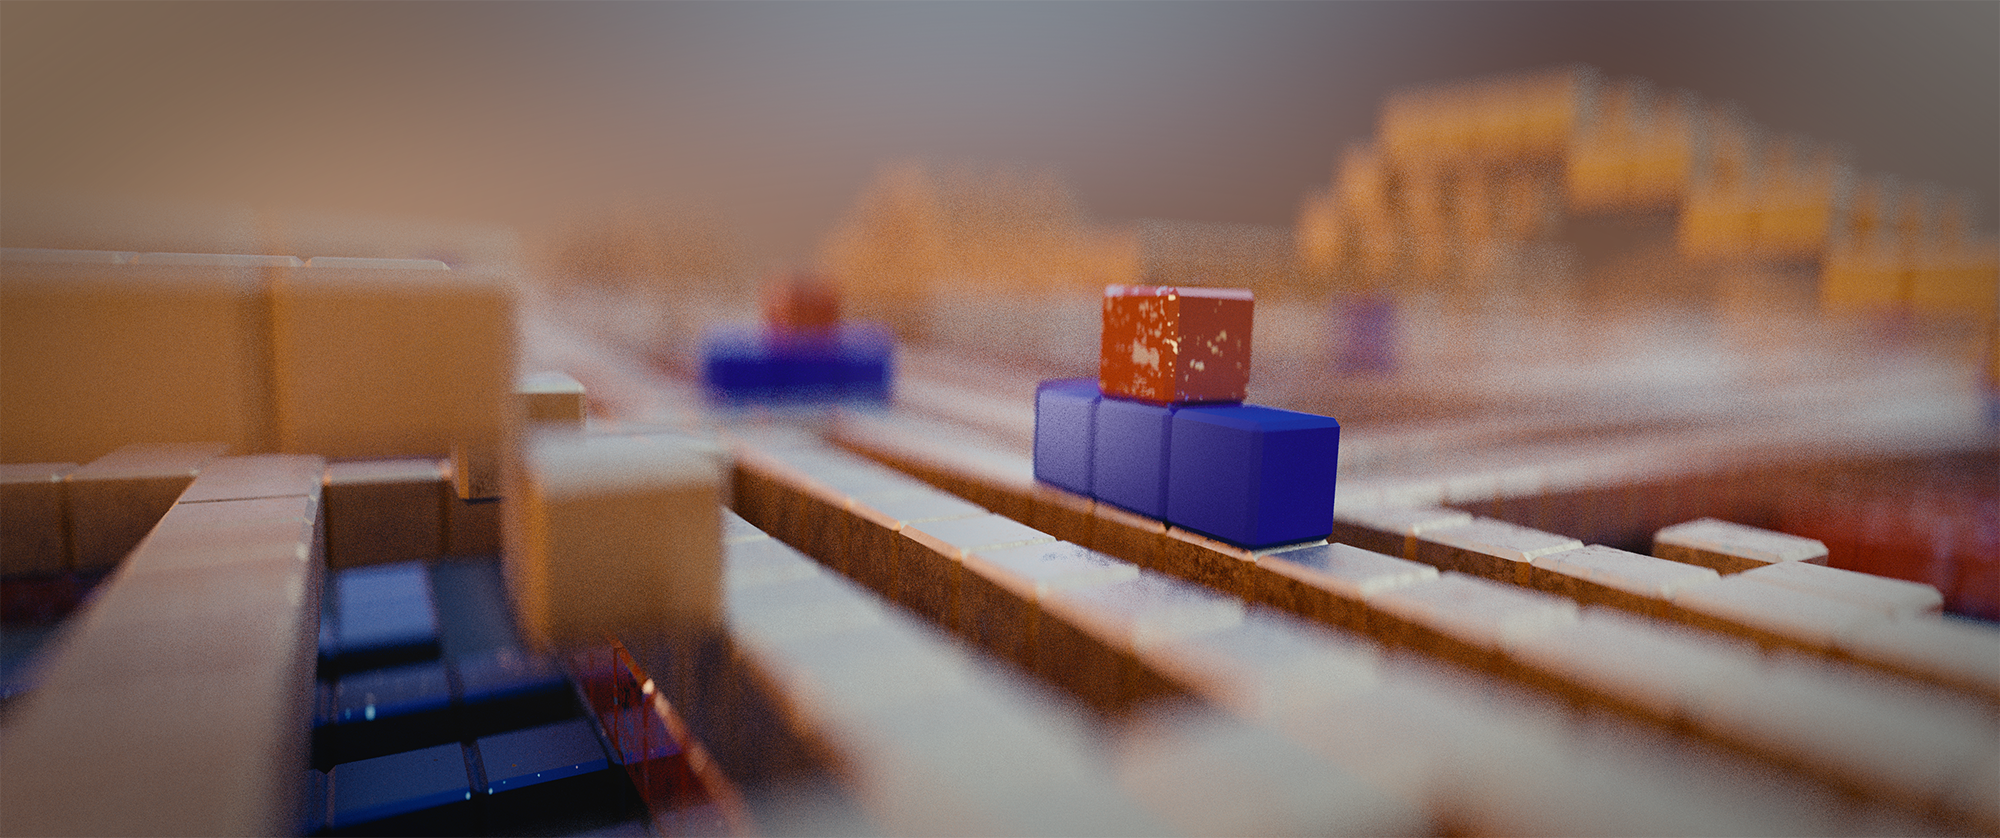
\includegraphics[width=\textwidth]{eliassembclose.png}
  \caption{\textit{Image Credit: Eli Gershenfeld 2016}}
  \label{fig:eliassembclose}
\end{figure}

\begin{figure}
  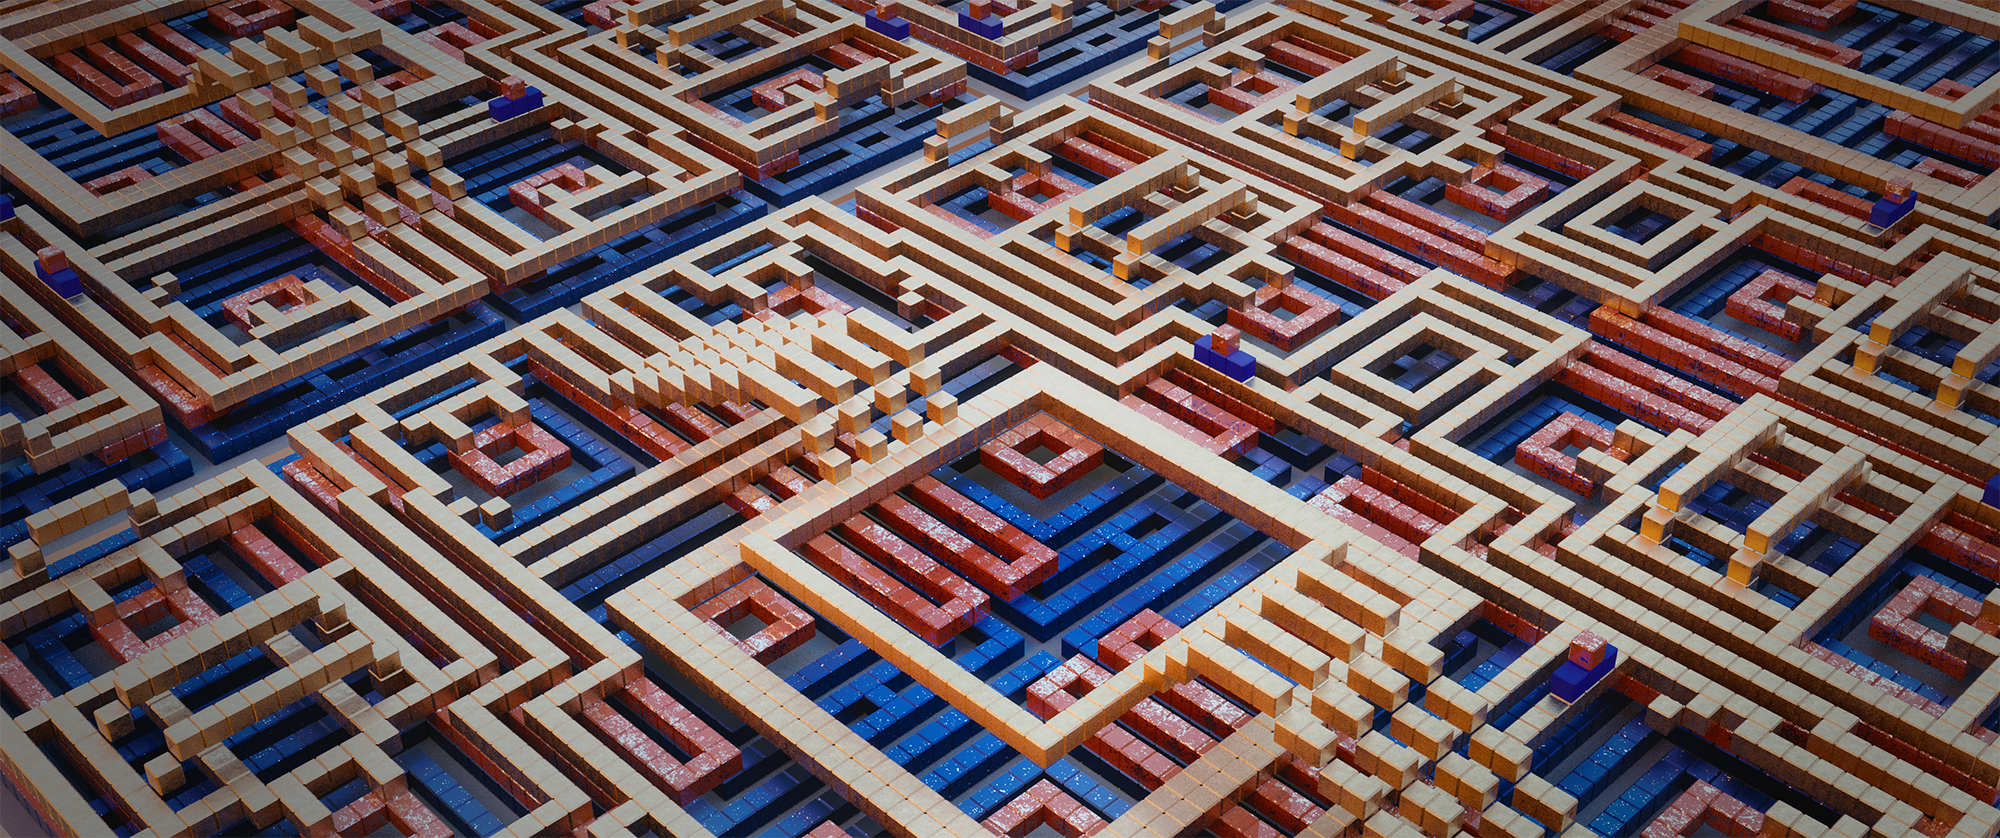
\includegraphics[width=\textwidth]{eliassembwide.png}
  \caption{\textit{Image Credit: Eli Gershenfeld 2016}}
  \label{fig:eliassembwide}
\end{figure}

\begin{figure}
  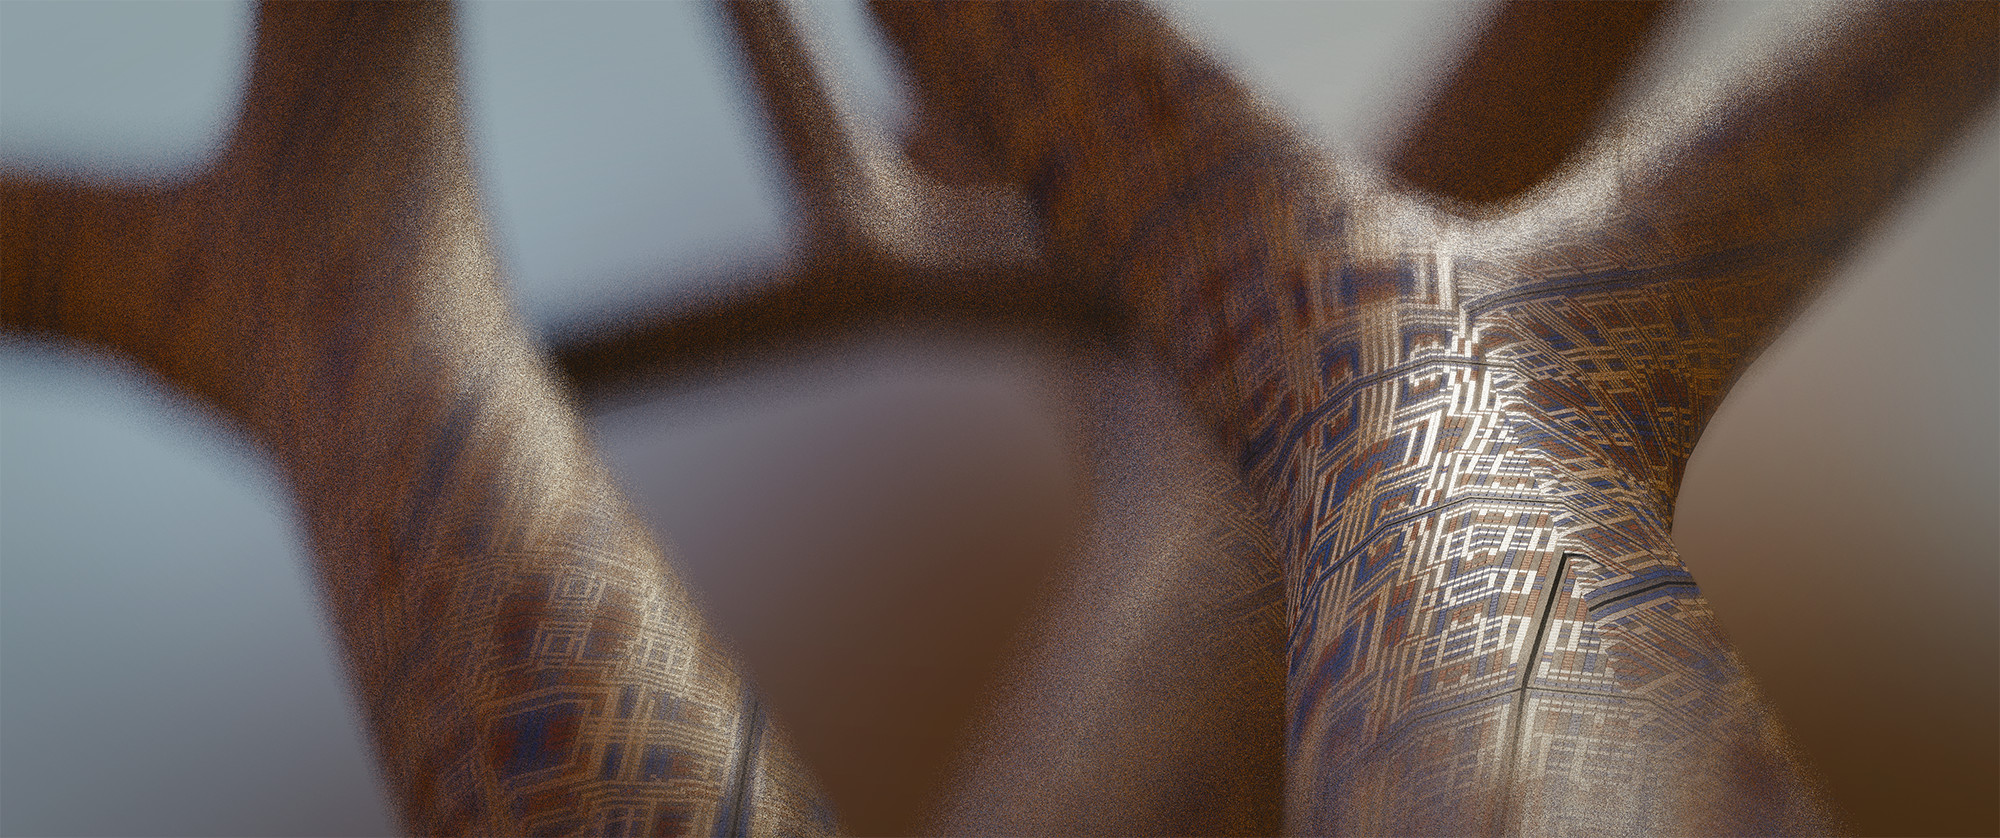
\includegraphics[width=\textwidth]{elibridgeclose.png}
  \caption{\textit{Image Credit: Eli Gershenfeld 2016}}
  \label{fig:elibridgeclose}
\end{figure}

\begin{figure}
  \includegraphics[width=\textwidth]{elibridgefull.png}
  \caption{\textit{Image Credit: Eli Gershenfeld 2016}}
  \label{fig:elibridgefull}
\end{figure}

\section{Computational Design Optimization}
